%TC:envir minted 1 xall 
%TC:envir algorithmic 1 xall

% Include tables in word count
%TC:envir table 0 word
%TC:envir tabular 1 word

% Include footnotes in word count
%TC:macro \footnote [text]
%TC:macro \footnotetext [text]

%TC:group minted 0 0
%TC:macro \mintinline [ignore]
%TC:macro \colb [ignore]
%TC:macro \hyperref [ignore]

\label{sec:2}
In preparation for my project, I learned a new programming language P4, explored how this language interacts with a software-defined data plane, studied the P4Pi networking platform, and worked through some provided example P4 programs. In \cref{sec:2.1} I define the notion of a software-defined router and explain why I chose this approach for my project. \cref{sec:2.2} and \cref{sec:2.3} introduce the DSL P4 and the networking platform P4Pi, respectively, and \cref{sec:2.4} explores the different components of the P4Pi platform and how they interact. Finally, \cref{sec:2.5} and \cref{sec:2.6} describe the project's starting point and my requirements analysis.



\section{Software-Defined Networking (SDN)}
\label{sec:2.1}

Software-Defined Networking (SDN) is an approach to network management that decouples the control plane software from the data plane hardware and moves the switch configuration mechanisms to software \cite{SDNPaper}. Network nodes based on this approach use generic hardware, which not only makes switch production easier and cheaper, but means that different network configurations can be built on top of a single piece of hardware. Providing customisable network infrastructure gives system admins control over configurations that were formerly baked into switch hardware \cite{SDN}. \cref{fig:prep-sdn} compares a traditional network and a software-defined network.

\begin{figure}[htbp]
  \centering
    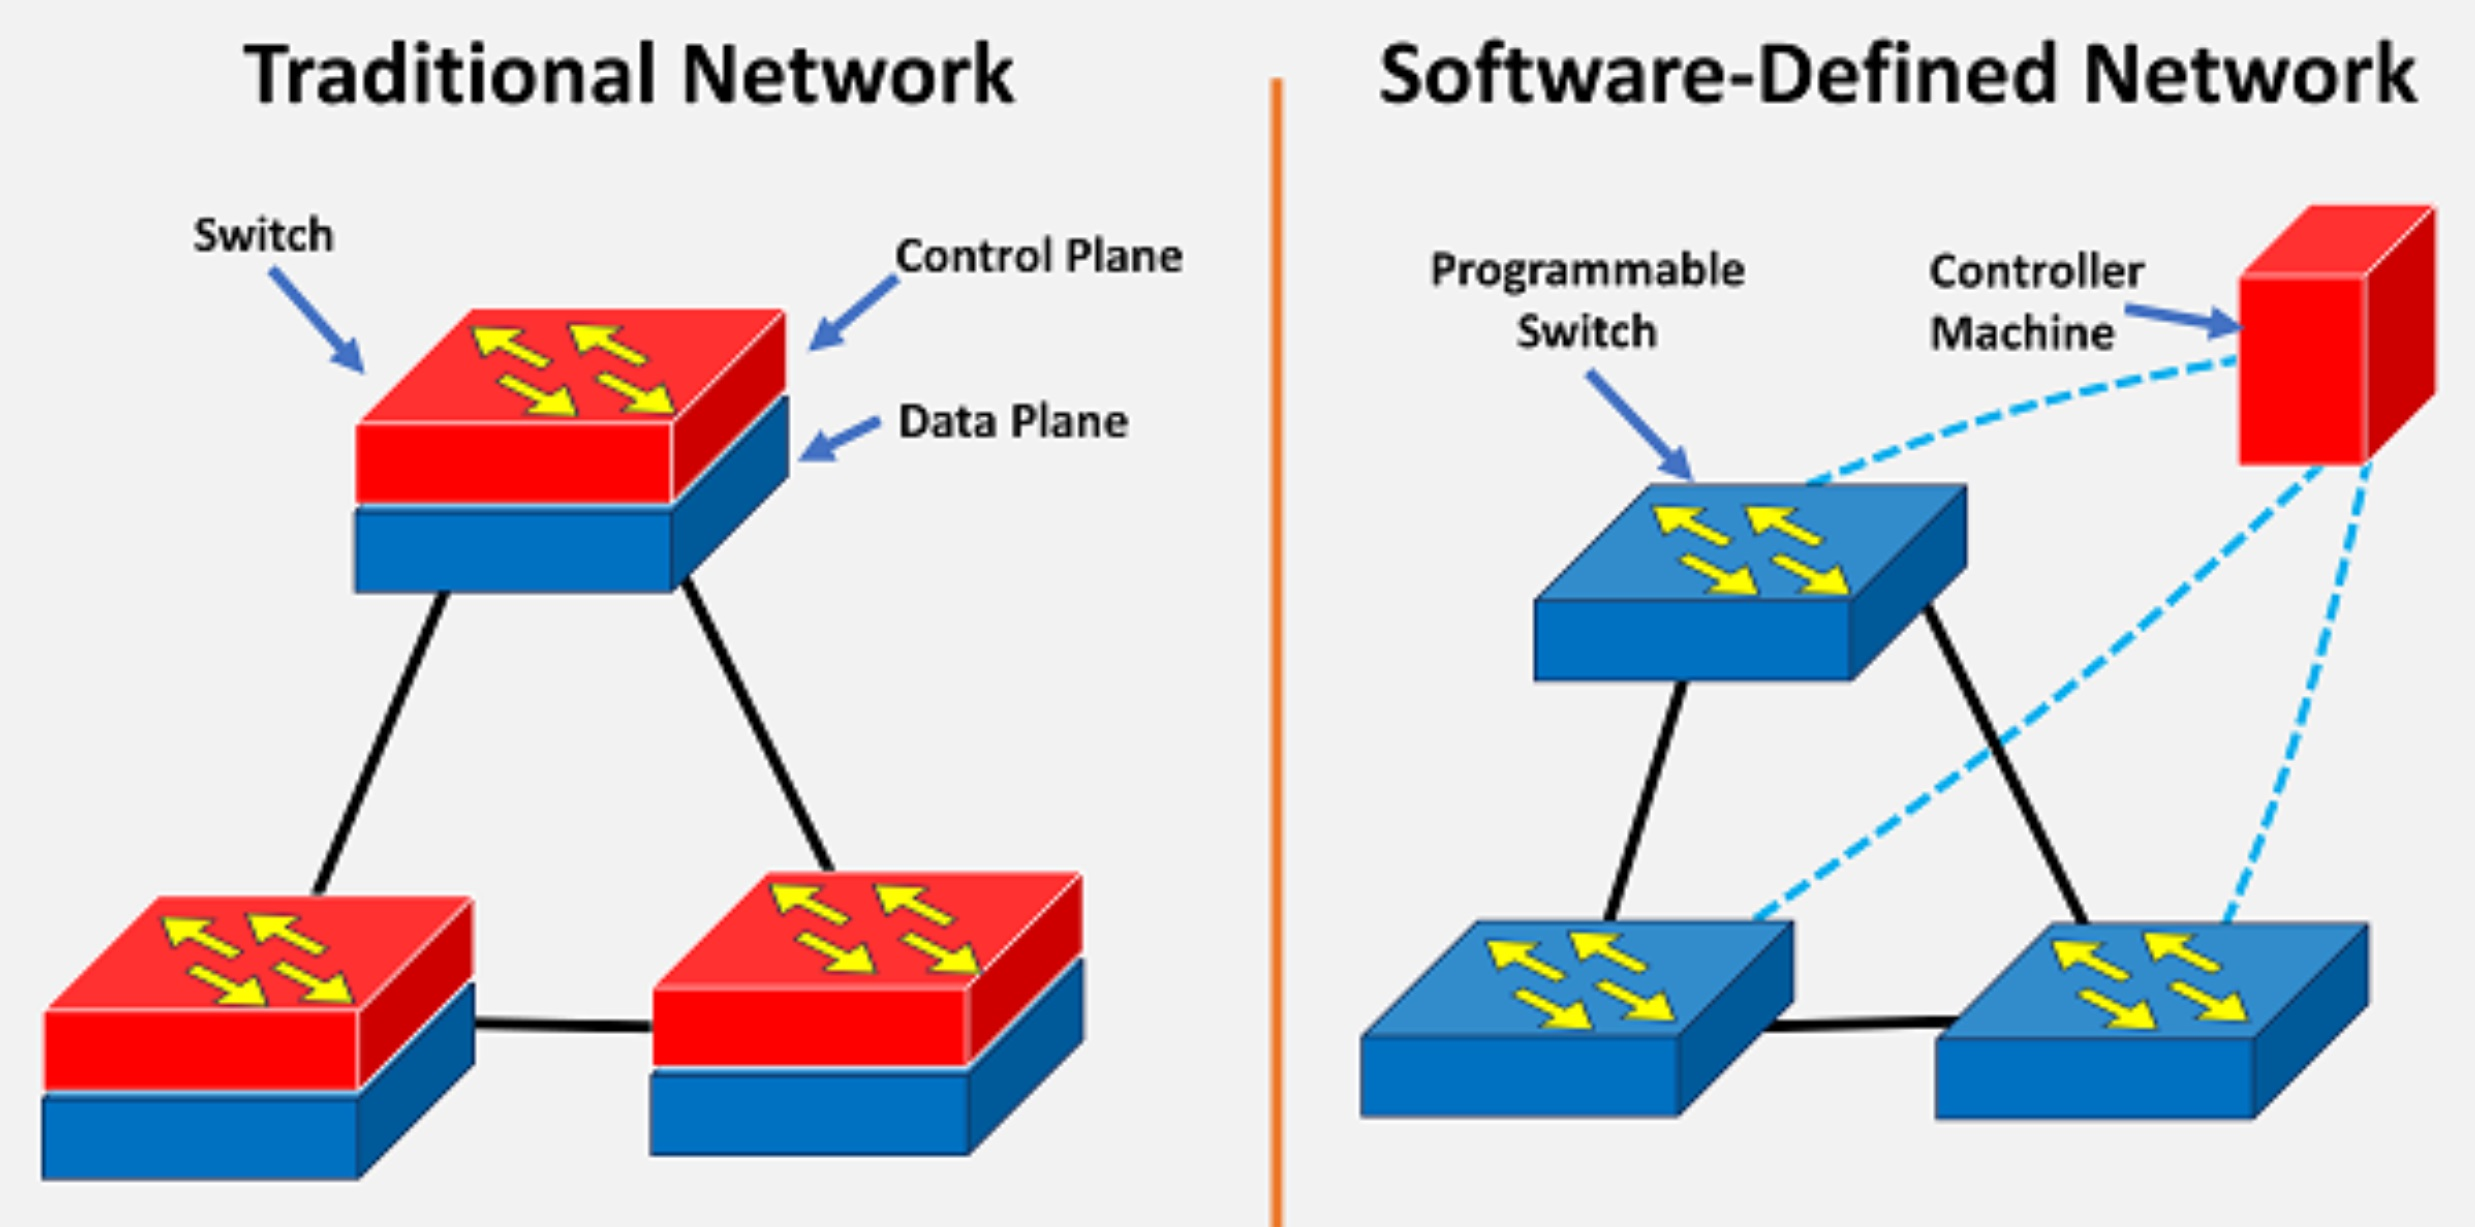
\includegraphics[width=0.8\textwidth]{figures/preparation/sdn.jpg}
     \caption{A comparison between a network consisting of traditional network \\ nodes and software-defined network nodes. Taken from \cite{SDNImage}.}
     \label{fig:prep-sdn}
\end{figure}

I chose to build my router on a software-defined platform because it provides more flexibility, a straightforward implementation pipeline, and real-time reconfiguration of network nodes. This made rerunning P4 code, changing network designs, and testing different data plane configurations much faster and simpler. It is also more affordable, since I  needed a general-purpose device to build my router on top of, rather than a specialised piece of hardware.



\section{P4 as a Network DSL}
\label{sec:2.2}
For my project, I chose the domain-specific language (DSL) P4 \cite{P4Paper}. P4 defines how packets are processed in the data planes of forwarding nodes, such as switches and routers. In accordance with the P4 language specifications, a packet-processing system capable of running P4 code is a P4 ‘target’, and a set of P4-programmable blocks are a P4 ‘architecture’ \cite{P4LangSpecs}.

P4 introduces a novel way of programming SDN nodes, which is flexible, expressive, and portable. The language can define data plane configurations of varying complexity to be run on a general-purpose target that does not have any fixed functionalities or knowledge of network protocols. A P4 program can be run on any target that supports the chosen architecture, regardless of the vendor that has produced it \cite{P4LangSpecs}.

P4 uses a set of core abstractions: header types, parsers, tables, actions, match-action units, and others. Functional blocks in the language can take three distinct parameter types: \texttt{in}, \texttt{inout} and \texttt{out}. The \texttt{in} parameter type is an immutable input; the \texttt{out} parameter type is initially undefined and can be written to; and the \texttt{inout} parameter type is a combination of both, i.e. initially defined and can be modified.

P4 uses most common data types, such as \texttt{void}, \texttt{int}, \texttt{string} and \texttt{bool}, along with \texttt{match\_kind} for table matching. It uses the types \texttt{bit<i>} and \texttt{int<i>} to define fixed-length variables of width \texttt{i}, as well as \texttt{varbit<i>} to define a variable of width between \texttt{0} and \texttt{i}. There are also a number of derived data types, such as \texttt{enum}, \texttt{header}, \texttt{header union}, \texttt{parser}, and \texttt{control} \cite{P4LangSpecs}. An example \texttt{control} block declaration is shown in \cref{fig:prep-matchaction}.

\begin{figure}[htbp]
  \centering
    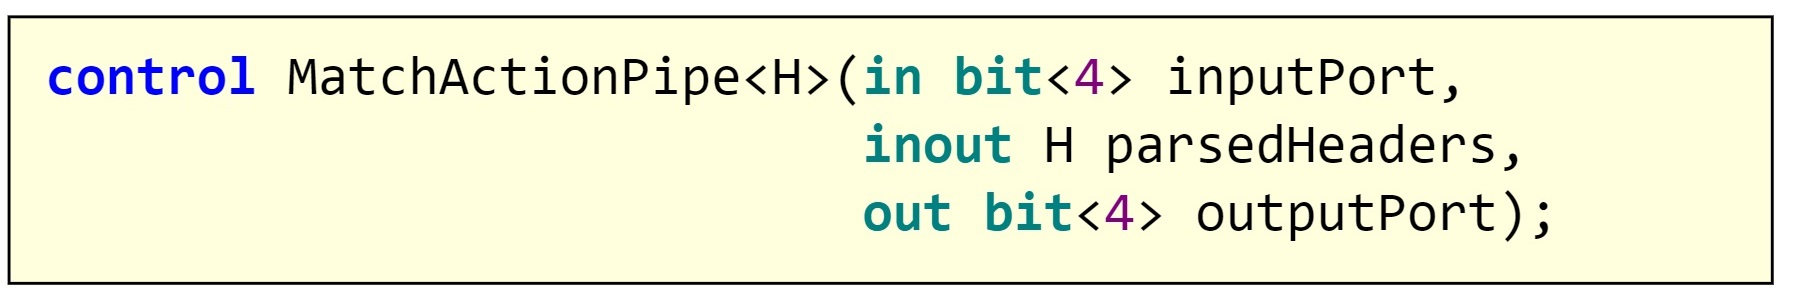
\includegraphics[width=0.7\textwidth]{figures/preparation/match_action.jpg}
     \caption{An example P4 control block declaration. Adapted from \cite{P4LangSpecs}.}
     \label{fig:prep-matchaction}
\end{figure}

A \texttt{header}, representing a packet header, is a collection of fields placed in a defined order. Headers need to have a maximum size, thus each field is either of type \texttt{bit<i>} or \texttt{varbit<i>}. If a header does not contain any \texttt{varbit<i>} type fields, then it is a fixed-size header, an example of which is shown in \cref{fig:prep-ethernet}. A \texttt{header union} represents a disjunction of multiple different headers, any of which could be placed at a point in the program where the header union is used.

\begin{figure}[hbtp]
  \centering
    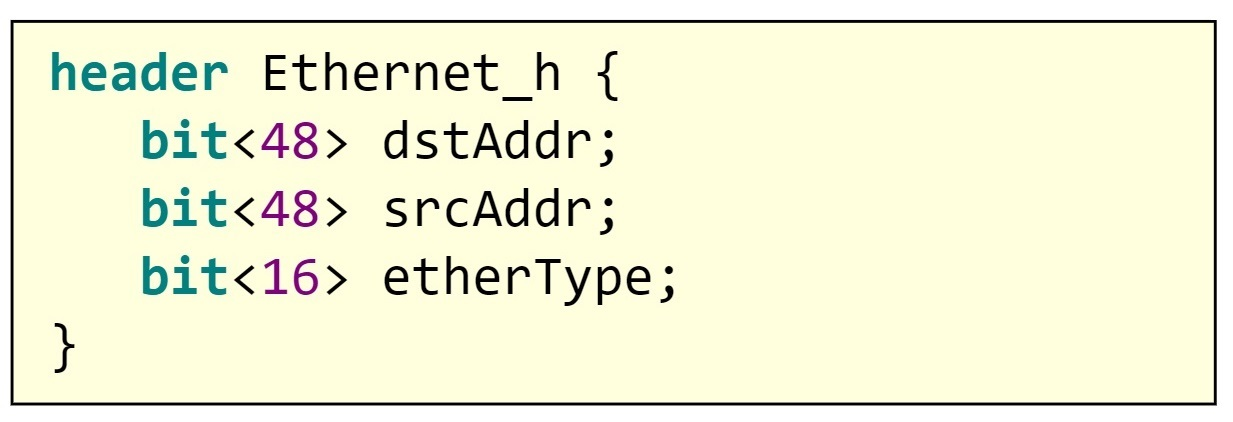
\includegraphics[width=0.5\textwidth]{figures/preparation/ethernet.jpg}
     \caption{An example Ethernet header. Adapted from \cite{P4LangSpecs}.}
     \label{fig:prep-ethernet}
\end{figure}

When a packet is being processed by a P4 program, it goes through three main stages: the \texttt{parser}, which extracts headers; the \texttt{match-action} pipeline, which manipulates the extracted headers; and the \texttt{deparser}, which prepends the updated headers. There are many ways that this pipeline can be further expanded upon, and in this dissertation I have additionally implemented \texttt{checksum verification} and \texttt{checksum update} stages.

A \texttt{parser} is a state machine with one starting state, \texttt{start}, and two final states, \texttt{accept} and \texttt{reject}. Each state is made up of statements that extract headers, lookup header fields and, optionally, define a transition to a different state. Accepted packets continue to the processing stages of the pipeline, whereas rejected packets are dropped. Parsers require an additional parameter type \texttt{packet\_in}, which represents the packet that has just entered the pipeline before headers are extracted. \cref{fig:prep-parser} is a \texttt{parser} declaration with one input and two outputs.

\begin{figure}[htbp]
  \centering
    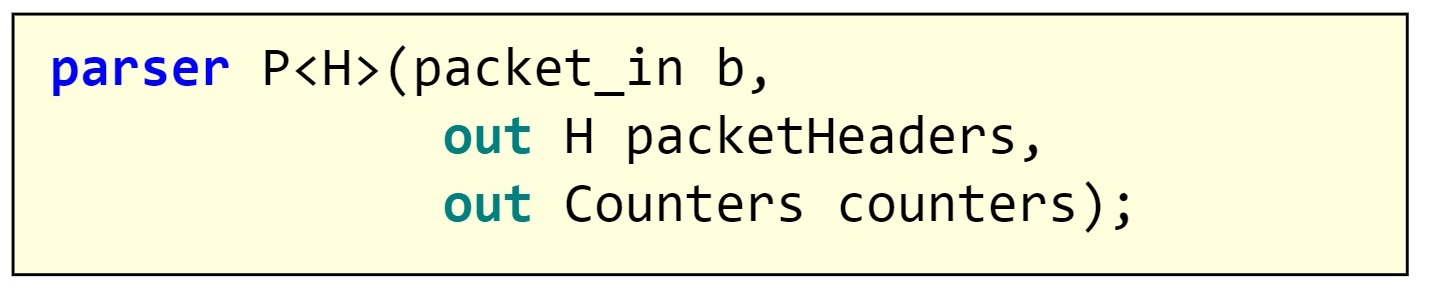
\includegraphics[width=0.55\textwidth]{figures/preparation/parser.jpg}
     \caption{An example \texttt{parser} declaration. Adapted from \cite{P4LangSpecs}.}
     \label{fig:prep-parser}
\end{figure}

A \texttt{control} block is a functional block used to manipulate headers extracted by the parser. It is made up of an \texttt{application} block, which defines the packet's control flow, \texttt{action} blocks, and \texttt{table} blocks. Actions are used to read and write processed data, whereas tables describe \texttt{match-action} units, i.e. units where a header field is matched to a table key to decide which action to take next. Each table entry consists of a key, an action ID and action data. Entries are checked from top to bottom, and if a match is encountered, the corresponding action is performed. A table for IPv4 forwarding using longest prefix match is shown in \cref{fig:prep-table}.

\begin{figure}[htbp]
  \centering
    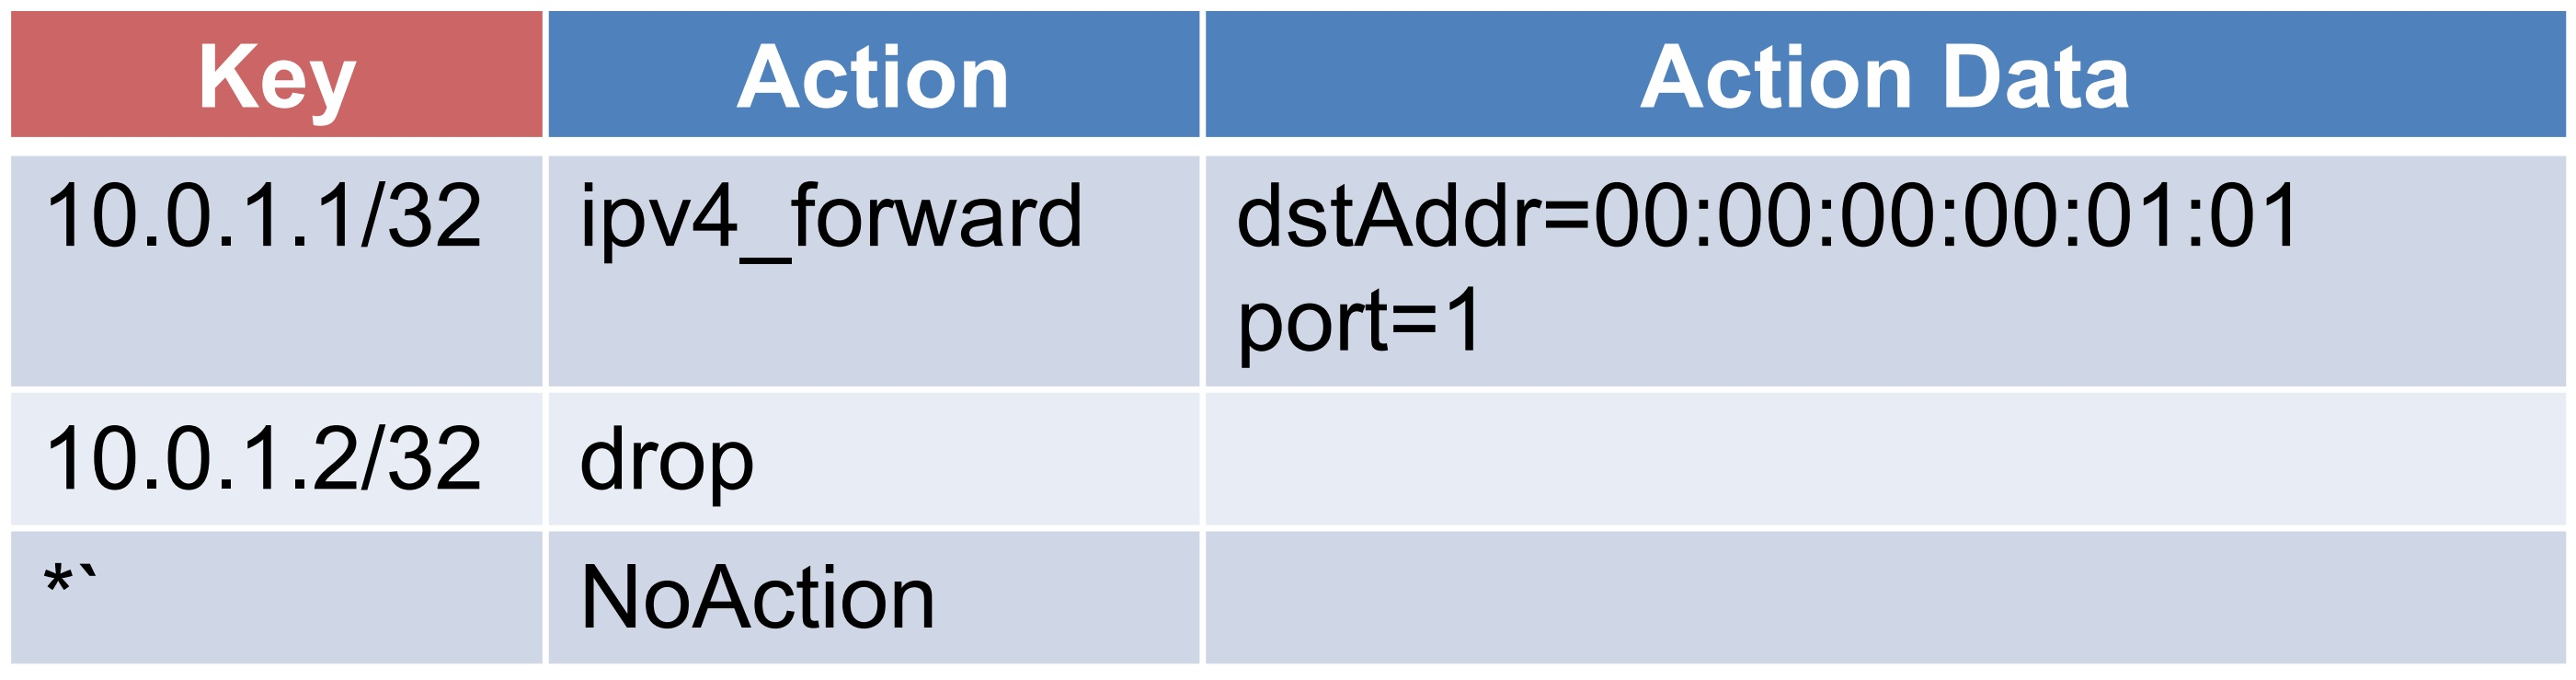
\includegraphics[width=0.55\textwidth]{figures/preparation/ipv4_table.jpg}
     \caption{An example \texttt{match-action} table. Taken from \cite{P4LangTutorial}.}
     \label{fig:prep-table}
\end{figure}

The \texttt{deparser} does not have its own derived type and is instead also performed in a \texttt{control} block, with the additional requirement that it must contain at least one parameter of type \texttt{packet\_out}. Similarly to how \texttt{packet\_in} represents the packet that has just arrived at the node, \texttt{packet\_out} defines the reconstructed packet that is sent back out into the network.

My project will not require any further P4 knowledge, but the language provides a wide variety of tools to build sophisticated packet control flow configurations beyond what I have discussed.



\section{P4Pi as an SDN Platform}
\label{sec:2.3}
P4Pi is an open source platform implemented on Raspberry Pi devices, which allows prototyping with P4. It provides an affordable hands-on method for research in the field of networking \cite{P4Pi}. The platform is available in a GitHub repository, which contains instructions on how to set up, install and configure the target \cite{P4Pi}. The repository defines a framework for running and testing P4 programs, which is outlined in \cref{sec:2.4} and also provides a few simple tutorials \cite{P4Pi}. I learned how to manipulate headers, perform table lookups, forward/drop packets, and use the Runtime Shell to dynamically update data plane tables.

I chose to conduct my project on this platform for multiple reasons: the required equipment is affordable and was available at the department; it is portable, which meant I could take it home and work on the project over the breaks; and most importantly, it allowed me to build a network of separate devices to route and track packets through, which helped me analyse the intricacies of a multi-host network. 



\section{Programming Framework}
\label{sec:2.4}

Programming a P4 target requires an understanding of how the different components of a packet-switching device interact with P4 code. \cref{fig:prep-framework} shows the stages a P4 program goes through before it runs on a target.

\begin{figure}[htbp]
  \centering
    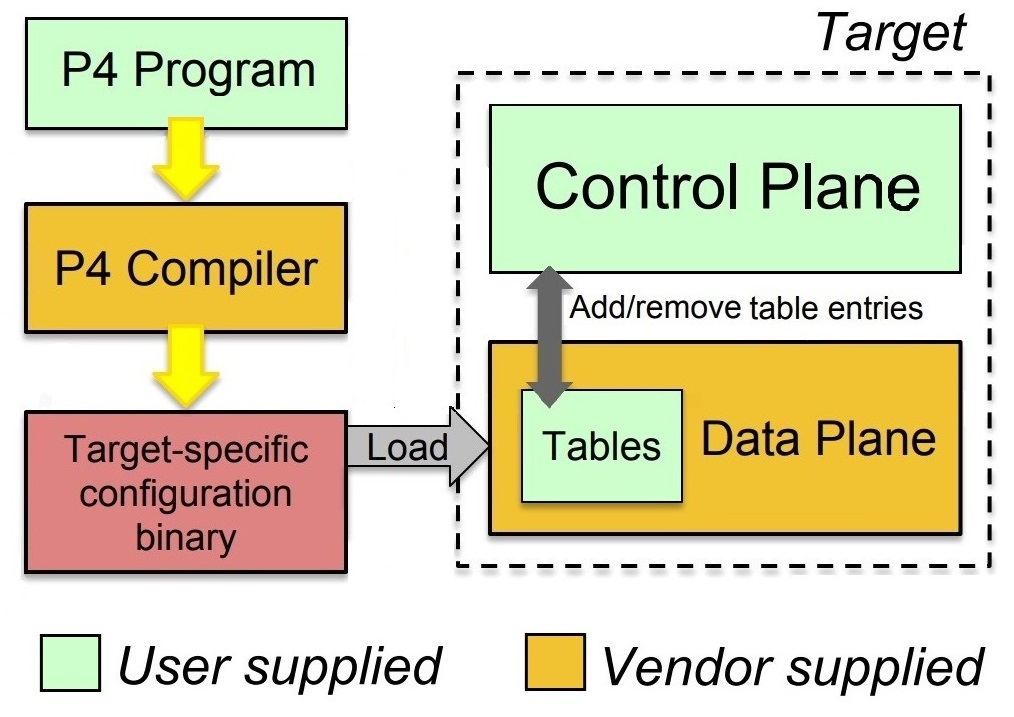
\includegraphics[width=0.5\textwidth]{figures/preparation/programming_target.jpg}
     \caption{Programming a P4 target. Adapted from \cite{P4LangTutorial}.}
     \label{fig:prep-framework}
\end{figure}

Every P4 program has to be written based on a defined architecture model, and every target has to abide by the behavioural model of a reference software switch. I define these notions in \cref{sec:2.4.1} and \cref{sec:2.4.2}, respectively. I describe how the P4 compiler produces a target-interpretable version of a P4 program in \cref{sec:2.4.3}, how it defines a control plane API in \cref{sec:2.4.4}. Finally, in \cref{sec:2.4.5}, I comment on how P4Pi interacts with external components, such as packet generators and packet sniffers.



\subsection{\textit{V1Model} Architecture}
\label{sec:2.4.1}

In my project, all P4 programs have been written abiding by the \textit{V1Model} architecture \cite{V1model}. A P4 architecture model defines a software template of a P4 program. In the V1Model, every program is made up of eight blocks of code: header definitions, parser, checksum verification, ingress processing, egress processing, checksum update, deparser, and a switch definition. All P4 code written by the user goes into one of these blocks and each function is required for the code to compile \cite{V1model}. \cref{fig:prep-v1arch} shows a simplified version of the packet processing pipeline defined by the \textit{V1Model}, and \cref{fig:prep-v1code} shows a P4 program structure split into the aforementioned eight code blocks. Each pipeline stage in \cref{fig:prep-v1arch} corresponds to one or more code block in \cref{fig:prep-v1code}.

\begin{figure}[htbp]
  \centering
    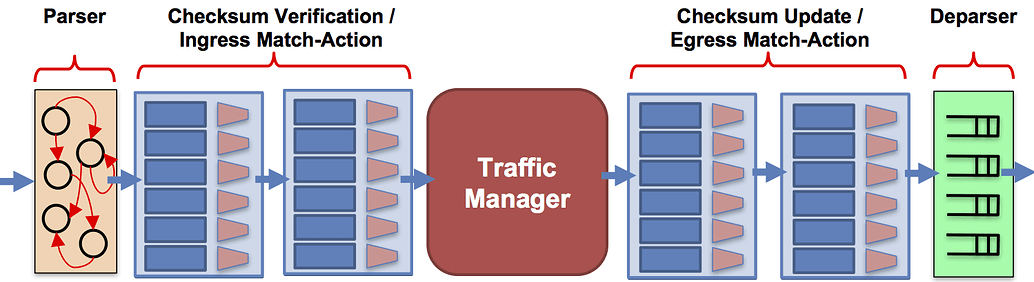
\includegraphics[width=0.8\textwidth]{figures/preparation/v1model_architecture.png}
     \caption{\textit{V1Model} pipeline. Taken from \cite{P4LangTutorial}.}
     \label{fig:prep-v1arch}
\end{figure}

\begin{figure}[htbp]
  \centering
    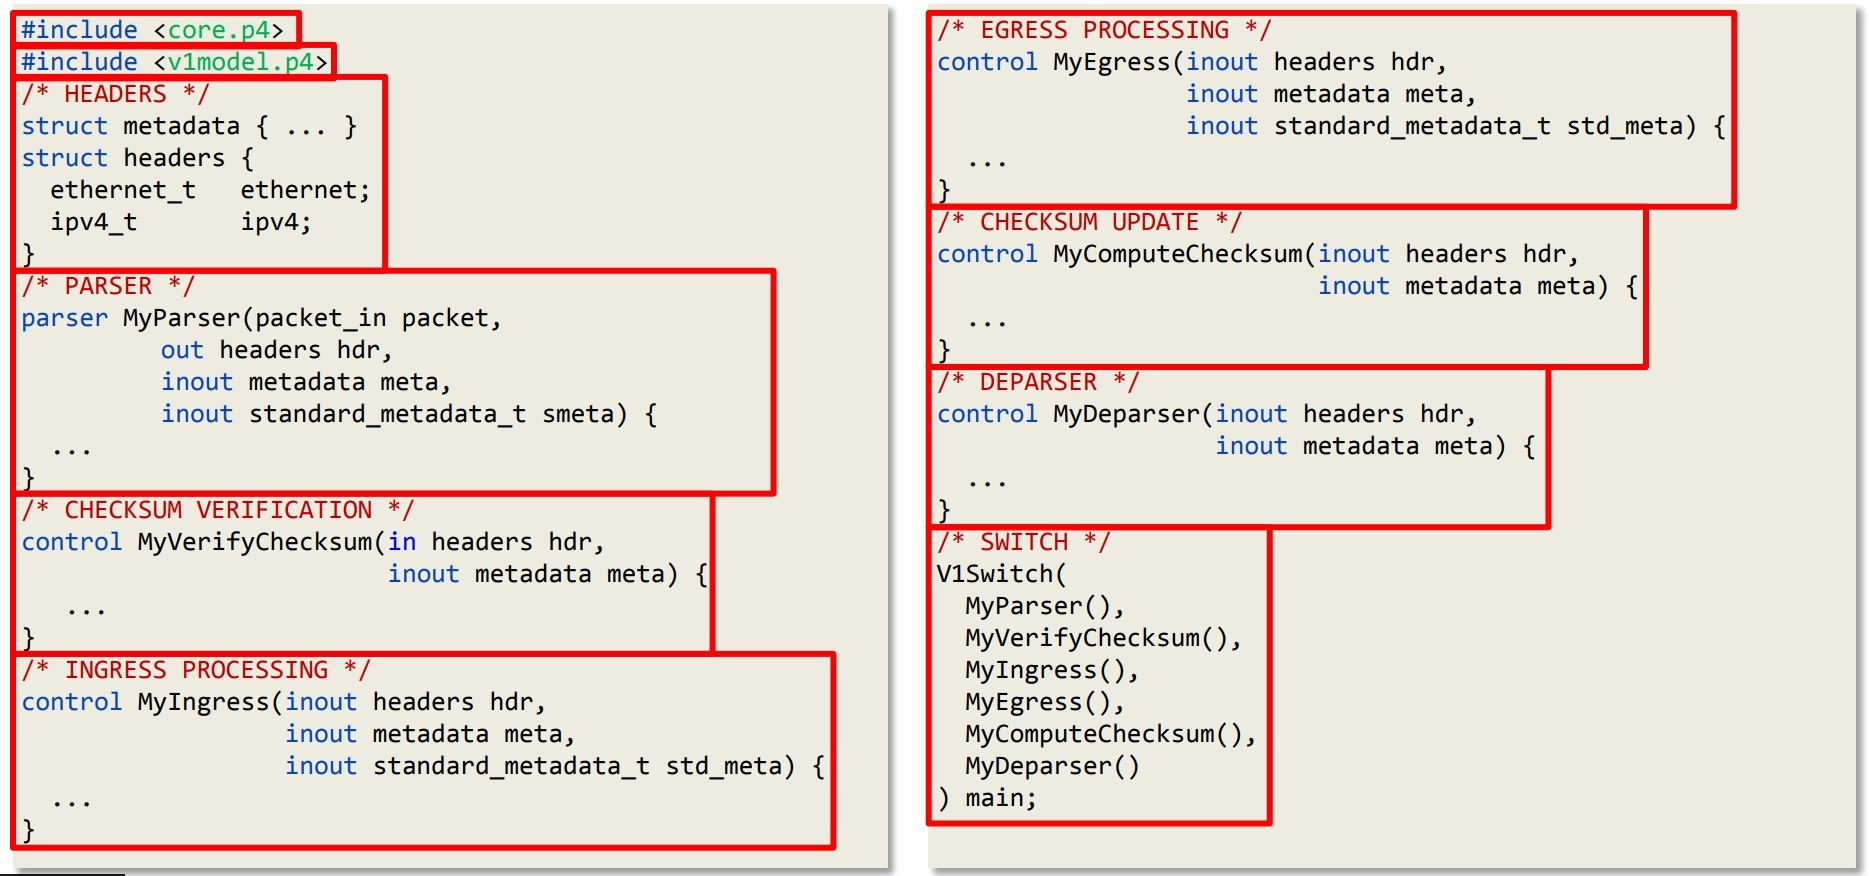
\includegraphics[width=0.8\textwidth]{figures/preparation/v1model_template.jpg}
     \caption{\textit{V1Model} code template. Taken from \cite{P4LangTutorial}.}
     \label{fig:prep-v1code}
\end{figure}



\subsection{\textit{Simple Switch} Target}
\label{sec:2.4.2}

I chose the \textit{simple switch} target for my project because it runs on a general-purpose CPU and offers all necessary functionalities. The \textit{simple switch} target is an implementation of the abstract \textit{BMv2} reference P4 software switch \cite{BMv2}. \textit{BMv2} is an abstract switch, i.e. it provides the necessary resources (such as how much memory is available) for a target to be implemented, but does not define a target implementation (e.g. using the memory to implement registers) \cite{P4LangTutorial}. The \textit{simple switch} target implements ingress and egress (de)parsers and control, as well as counters, actions, a checksum function, packet buffers with replication engines, and many more. It also offers runtime support for updating the control plane without requiring recompilation of the P4 program \cite{BMv2target}. \cref{fig:prep-relation} shows the relationship between a P4 program, the \textit{V1Model} architecture model, the \textit{simple switch} target implementation, and the \textit{BMv2} behavioural model.

\begin{figure}[htbp]
  \centering
    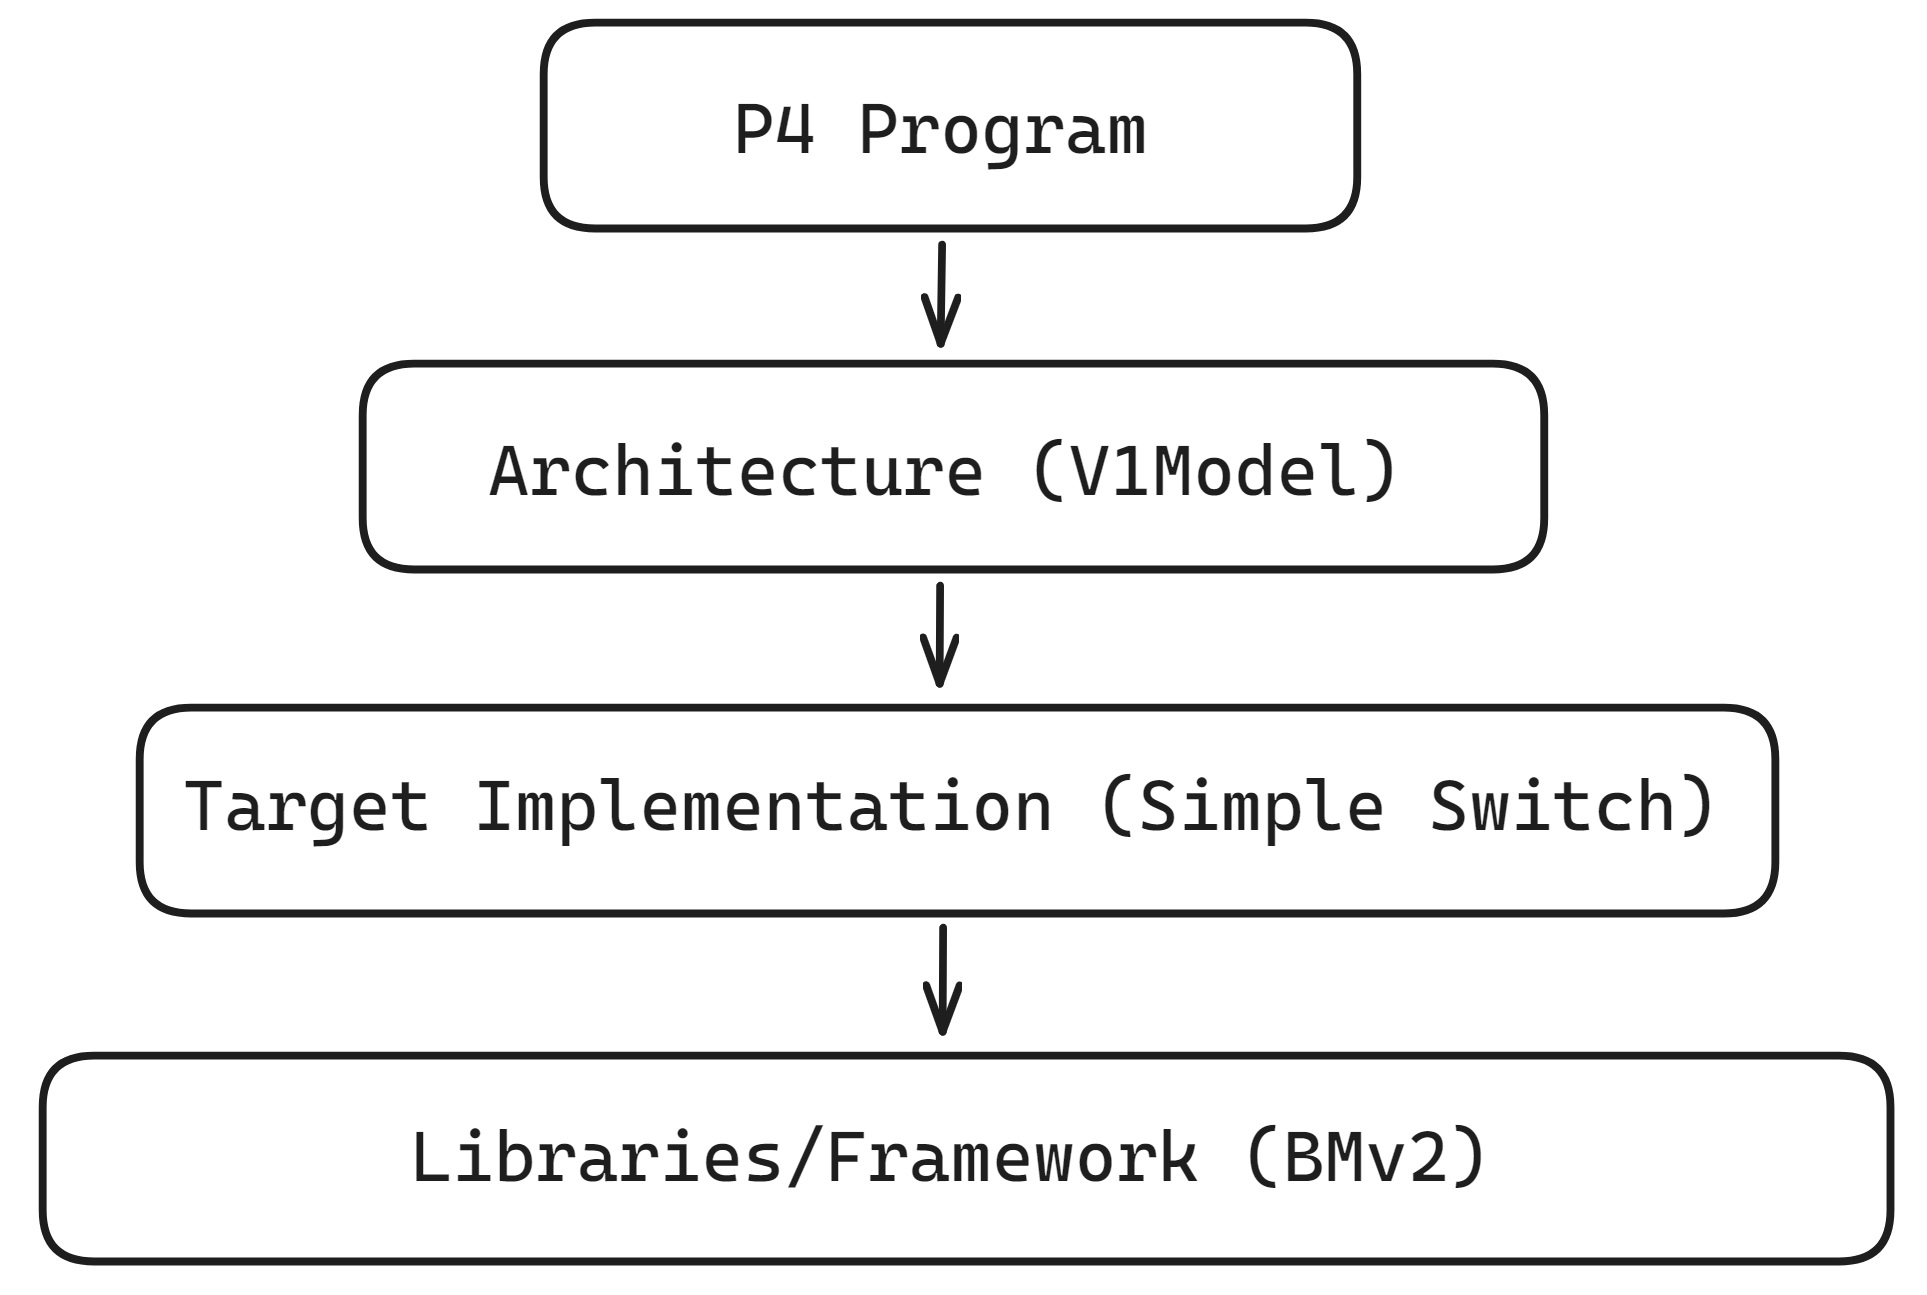
\includegraphics[width=0.45\textwidth]{figures/preparation/control_flow.jpg}
     \caption{Relating concepts. Adapted from \cite{P4Architecture}.}
     \label{fig:prep-relation}
\end{figure}



\subsection{P4 Compiler}
\label{sec:2.4.3}

The default reference compiler for the P4 language is \textit{p4c}, which provides a standardised modular frontend and midend for the compiler. To produce a fully-functional P4 Compiler, \textit{p4c} must be combined with a target-specific backend. The provided backend for the \textit{simple switch} target is \textit{p4c-bm2-ss} \cite{P4Compilers}.

The \textit{simple switch} P4 compiler takes four arguments:
\begin{itemize}[topsep=0pt]
\item \textit{BMv2} – the abstract switch model;
\item \textit{v1Model} – the architecture model;
\item \texttt{p4-16} – the P4 version the program was written in;
\item a \texttt{.p4} file – the P4 program to be compiled;
\end{itemize}

and outputs two files:
\begin{itemize}[topsep=0pt]
\item \texttt{.p4i} – contains the preprocessor output;
\item \texttt{.json} – data plane configurations in the file format \textit{BMv2} targets require as input.
\end{itemize}

The \texttt{.json} file can then be run on the \textit{simple switch} target. For more details on how to run a P4 program on the P4Pi platform, see Appendix A \cite{P4Pi}. 

\subsection{\textit{Simple Switch CLI}}
\label{sec:2.4.4}

The target's command line interface, \textit{simple switch CLI} allows dynamic inspection, addition, deletion, and modification of the tables defined by the P4 program. Each table entry consists of a key-action pair where the action tells the switch how to proceed upon a key match. For a brief overview of commands that can be used in the CLI, see Appendix B \cite{P4LangTutorial}.




\subsection{External Components}
\label{sec:2.4.5}

Once a program has been compiled and loaded into the P4Pi switch, it can interact with external components. A packet generator (e.g. Scapy \cite{Scapy}) can be used to send packets to the target. Packets go through the port interface and into the \textit{V1Model} pipeline, where they are manipulated as defined by the P4 program data plane configurations. A packet sniffer (e.g. Wireshark \cite{Wireshark}) can then be used inspect the packets once they have been processed and outputted. Running in parallel, the target's CLI can dynamically update the data plane tables. Changes made through the CLI take effect immediately and new packet processing behaviour is then observed. \cref{fig:prep-overview} illustrates the described interactions.

\begin{figure}[htbp]
  \centering
    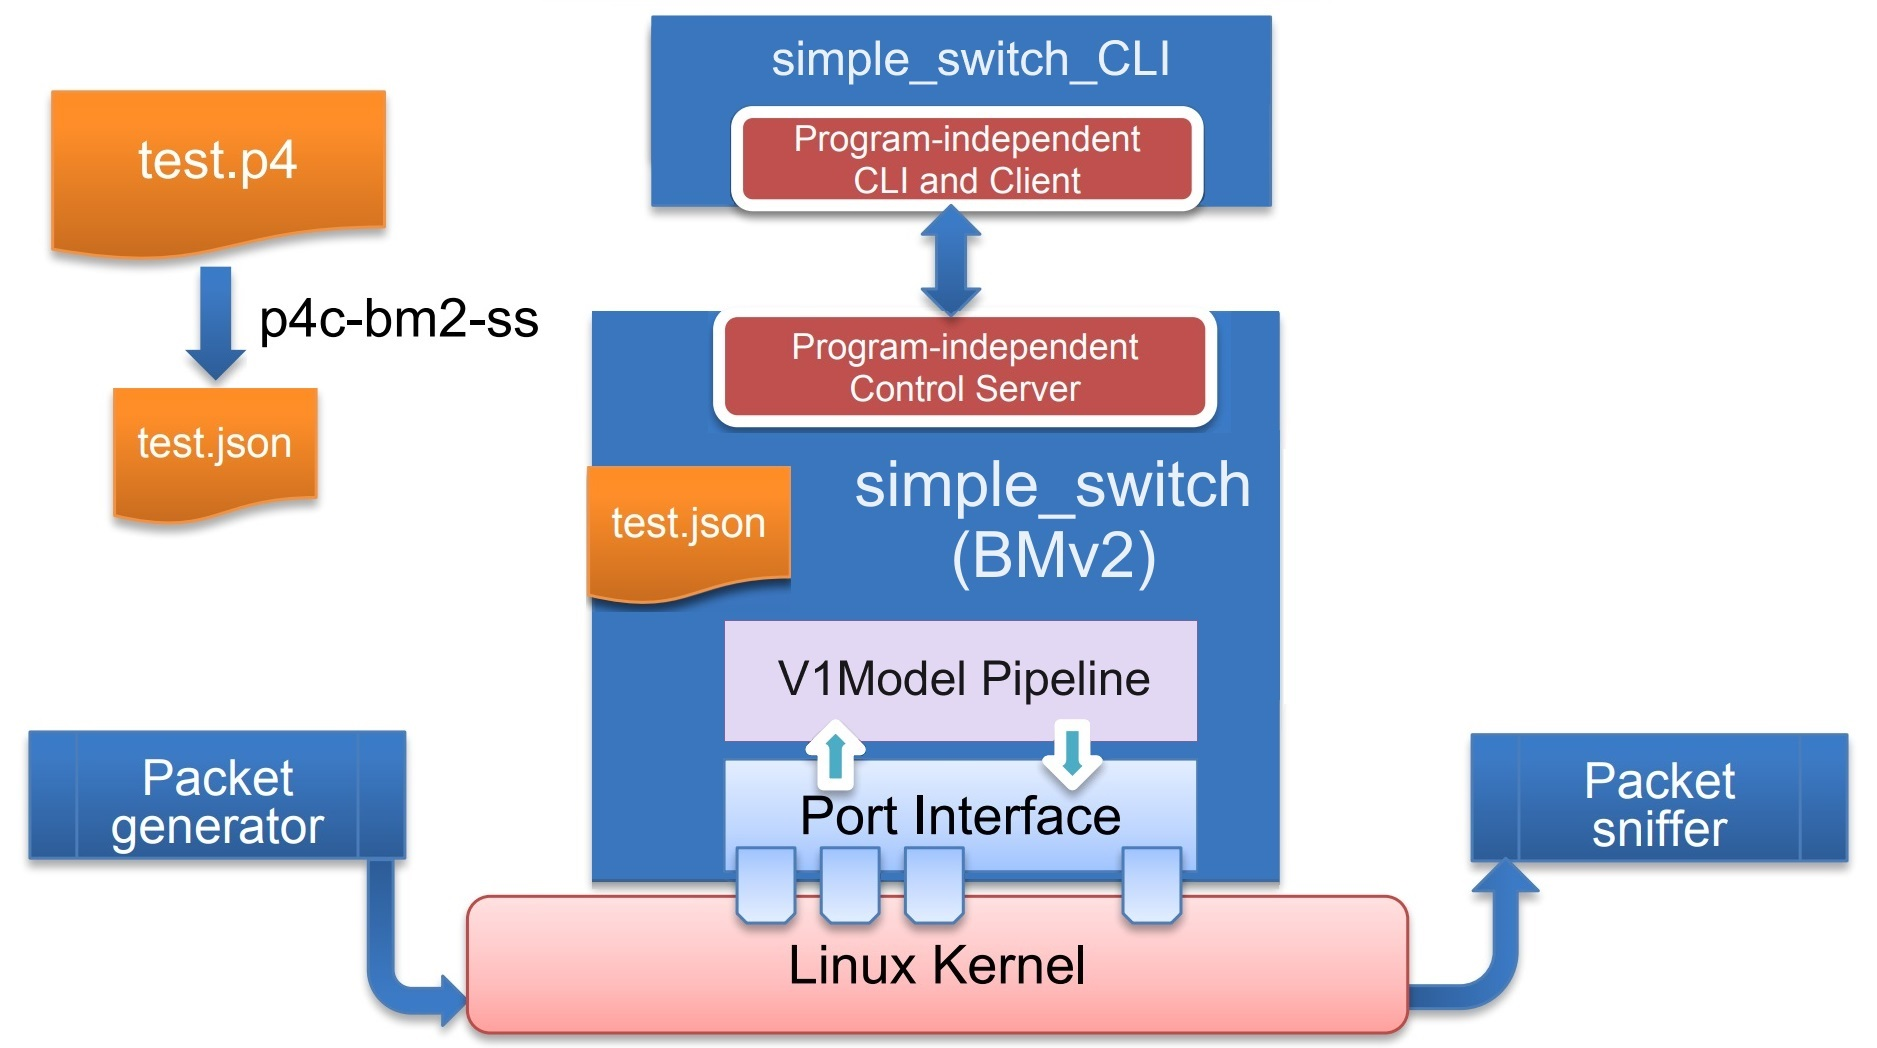
\includegraphics[width=0.8\textwidth]{figures/preparation/overview.jpg}
     \caption{Interaction with external components. Adapted from \cite{P4LangTutorial}.}
     \label{fig:prep-overview}
\end{figure}




\section{Starting Point}
\label{sec:2.5}
The initial P4Pi repository contained a P4 architecture (\textit{V1Model}), a P4 compiler, a P4 target (\textit{simple switch}), a target-specific Runtime Shell (\textit{simple switch CLI}), and some example IPv4 functionalities, such as forwarding, ARP Reply, and Echo Reply.

The aim of my project is to build an IPv6 router prototype. The core objective is for the router to support parsing, header manipulation, and forwarding of IPv6 packets. Two of my extensions are to add ICMPv6 and NDP functionalities (the equivalent of IPv4’s ICMP and ARP, respectively). The final extension takes a simple P4 IPv4 router (adapted from the P4Pi repository) and merge it with my IPv6 router to build a dual-stack router prototype, which can process both IPv4 and IPv6 packets.



\section{Requirements Analysis}
\label{sec:2.6}

My project required hardware, which I obtained from my supervisor: three Raspberry Pis, three SD cards, Ethernet cables, and Ethernet-to-USB adaptors. I occasionally used my college's computer room to set up multiple monitors, mouses, and keyboards in order to attach each Raspberry Pi to its own screen.

I set up a GitHub repository to regularly push all my code to and adhered to P4 standards when writing and formatting my code. I used the iterative agile methodology for code development in order to break down my work into tasks that can be achieved within a fortnight. The project was built using test-driven development. Using the packet analyser Wireshark \cite{Wireshark}, I observed packet formats and exchanges in a working network, and based my router behaviour on them. I used bespoke testing on known test traffic to evaluate the correctness and performance of my P4 programs.

\cref{fig:prep-req} shows all required functionalities, grouped into core objectives and three extensions. This diagram is not intended as a packet dataflow. It is intended to show the dependencies between router components. An arrow from Block A to Block B means that Block A needs to be implemented in order for Block B to work. All tasks have been successfully completed.

\begin{figure}[hbtp]
  \centering
    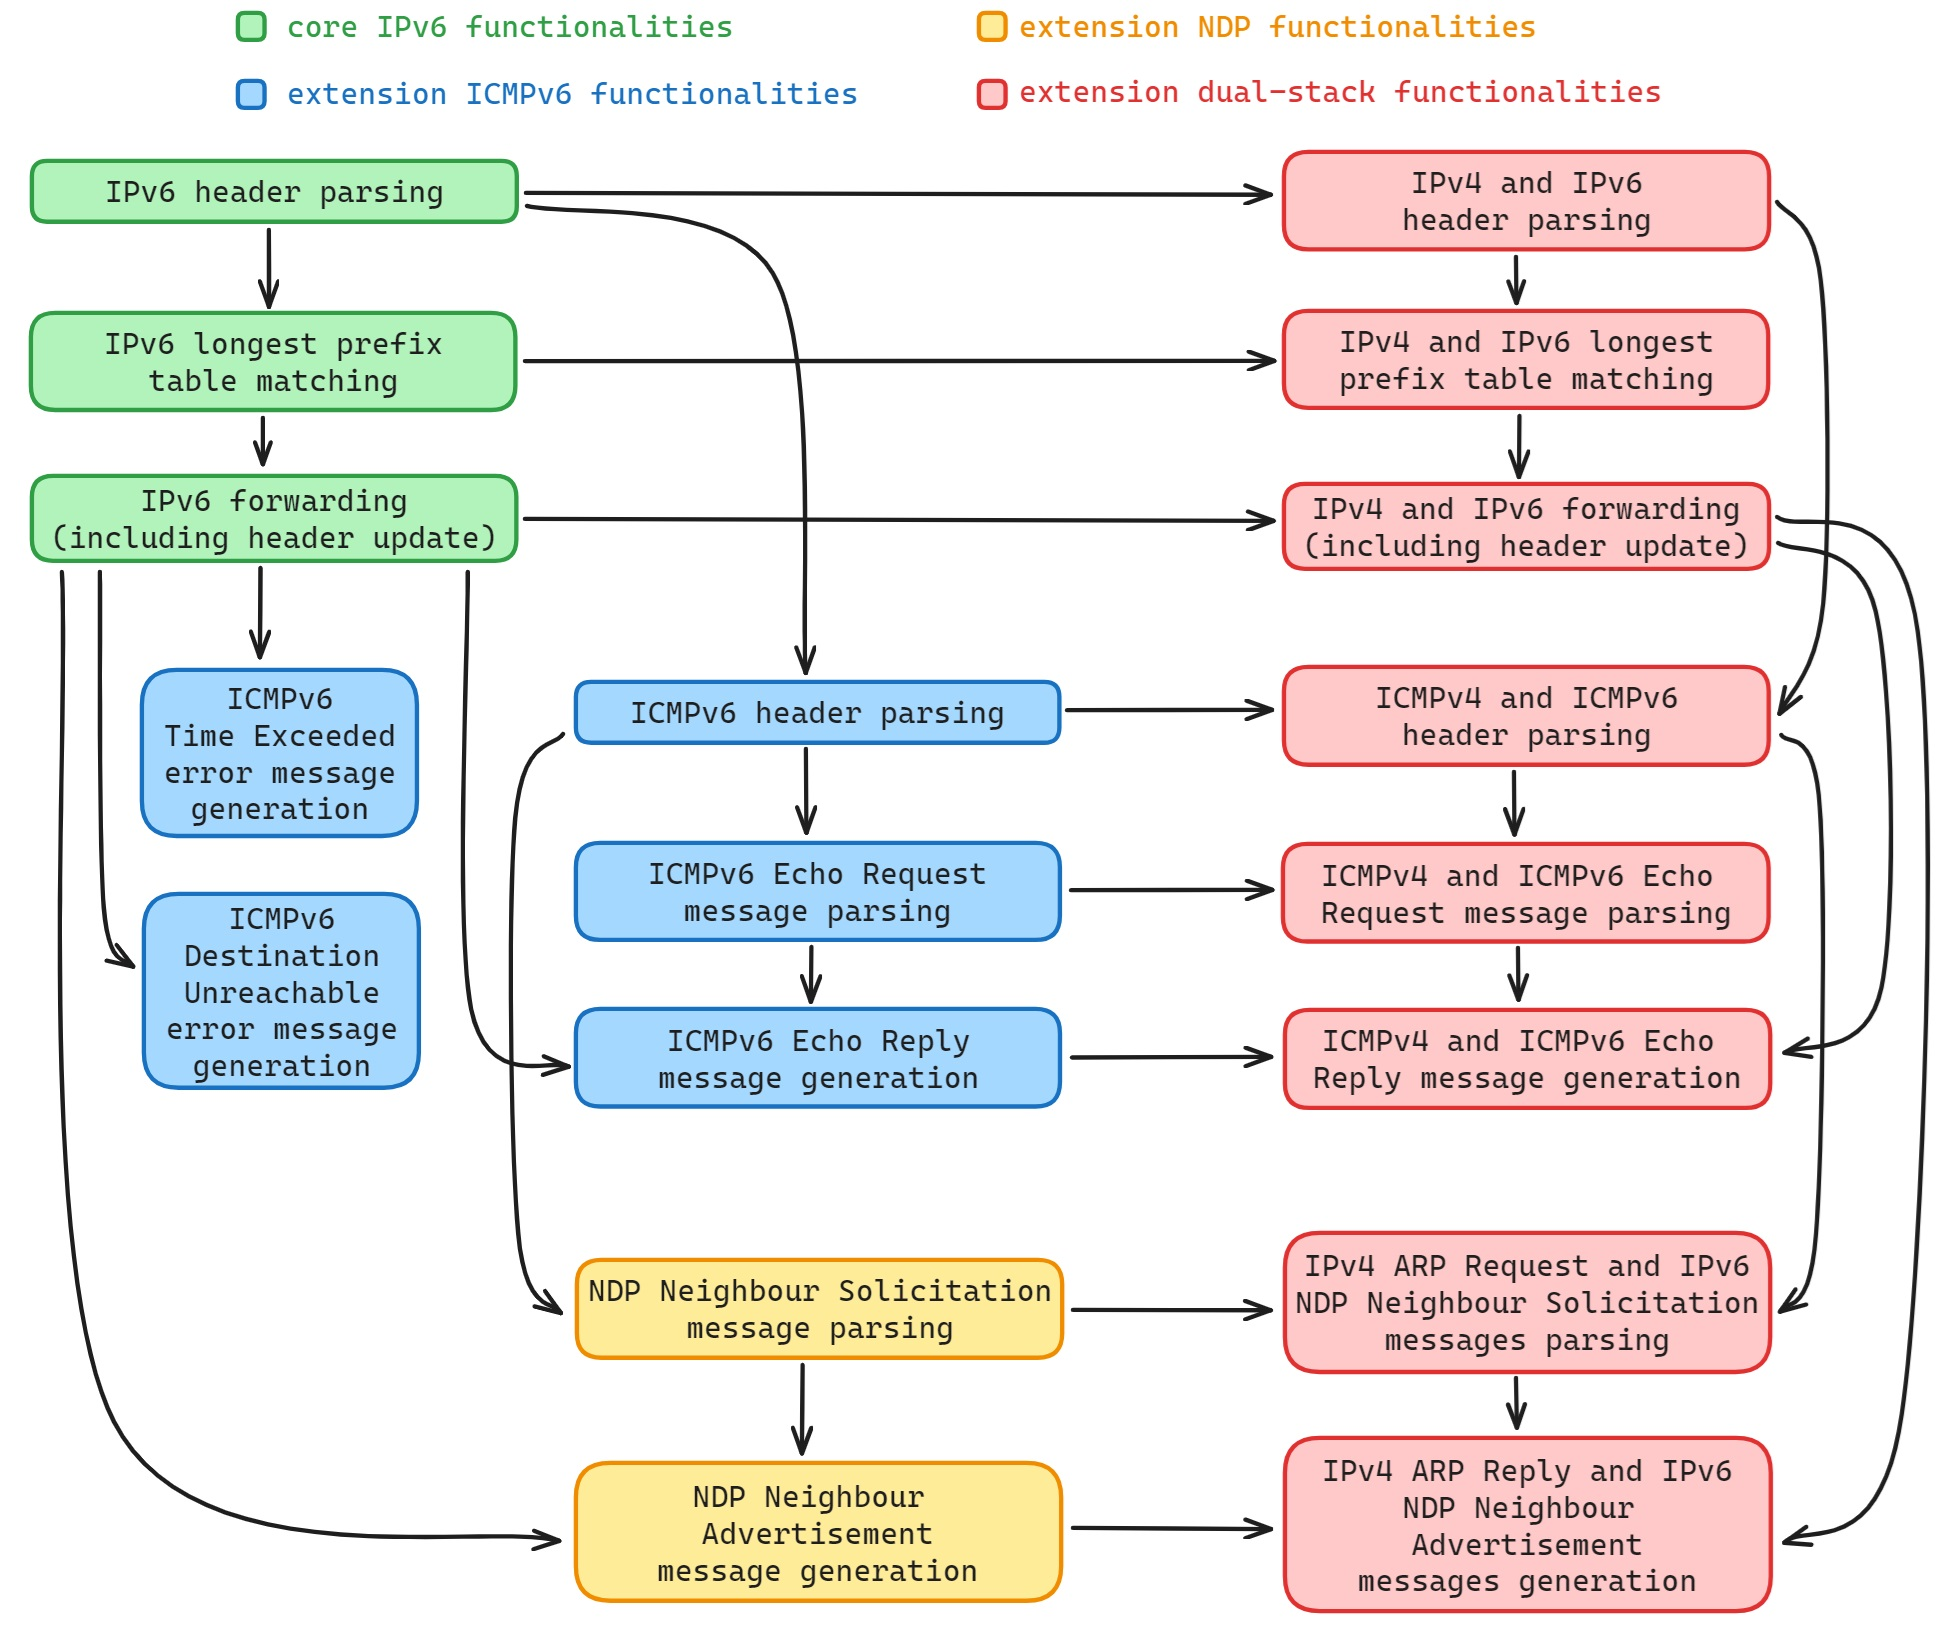
\includegraphics[width=1\textwidth]{figures/preparation/req_analysis.jpg}
     \caption{Dependency diagram between router functionalities.}
     \label{fig:prep-req}
\end{figure}